\documentclass{standalone}
\usepackage{pgfplots}
\usepackage[charter]{mathdesign}
\begin{document}
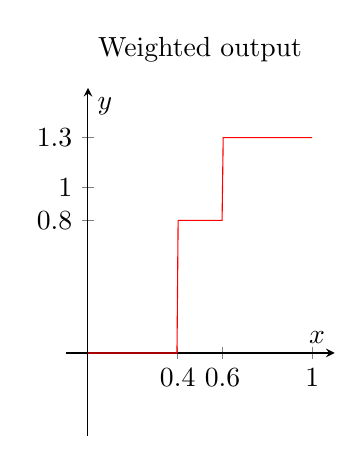
\begin{tikzpicture}[x={(2cm,-0.3cm)},y={(-0.1cm,2cm)},declare function={step(\x,\s)=0.5*(sign(\x-\s)+1);}]
	\begin{axis}[width=5cm,height=6cm,xlabel={$x$},ylabel={$y$},title={Weighted output},xtick={0,0.4,0.6,1},ytick={0,0.8,1,1.3},xmax=1.1,xmin=-0.1,ymin=-0.5,ymax=1.6,axis x line=middle,axis y line=middle]
		\addplot[red,domain=0:1, samples=200]{0.8*step(x,0.4)+0.5*step(x,0.6)};
	\end{axis}
%	\clip (-0.5,-0.5) rectangle ++(2,3.5);
%	\draw[-latex] (0,-0.5) -- (0,2.2) node[left] {$y$};
%	\draw[-latex] (-0.25,0) -- (1.2,0) node[below] {$x$};
%	\draw[red,thick] (0,0) -- ++(0.4,0) coordinate (s1) -- ++(0,0.6) coordinate (s2) node[midway,sloped,above] {$h_1$} -- ++(0.2,0) coordinate (s3) -- ++(0,1.2) coordinate (s4) node[midway,sloped,above] {$h_2$} -- ++ (0.2,0);
\end{tikzpicture}
\end{document}
		